%==============================================================================
% Chapitre 53 - Les munitions de chasse
%==============================================================================

\section{Introduction}

La chasse constitue l'une des principales applications civiles des armes à feu.

Au fil du temps, de nombreuses munitions ont été développées afin de répondre
à des besoins très différents selon le type de gibier recherché.

Les contraintes rencontrées diffèrent souvent de celles du domaine militaire.

\begin{aretenir}

Une munition de chasse doit permettre un prélèvement efficace tout en limitant
autant que possible les souffrances de l'animal.

\end{aretenir}

\section{Diversité des situations}

Les conditions de chasse peuvent varier considérablement.

Les paramètres à prendre en compte incluent notamment :

\begin{itemize}
    \item la taille du gibier ;
    \item la distance de tir ;
    \item l'environnement ;
    \item le type d'arme utilisée.
\end{itemize}

Cette diversité explique l'existence d'un grand nombre de munitions.

\section{Petit gibier et grand gibier}

On distingue généralement :

\begin{itemize}
    \item le petit gibier ;
    \item le grand gibier.
\end{itemize}

Les caractéristiques recherchées pour les munitions diffèrent fortement entre
ces deux catégories.

\begin{figure}[htbp]
\centering

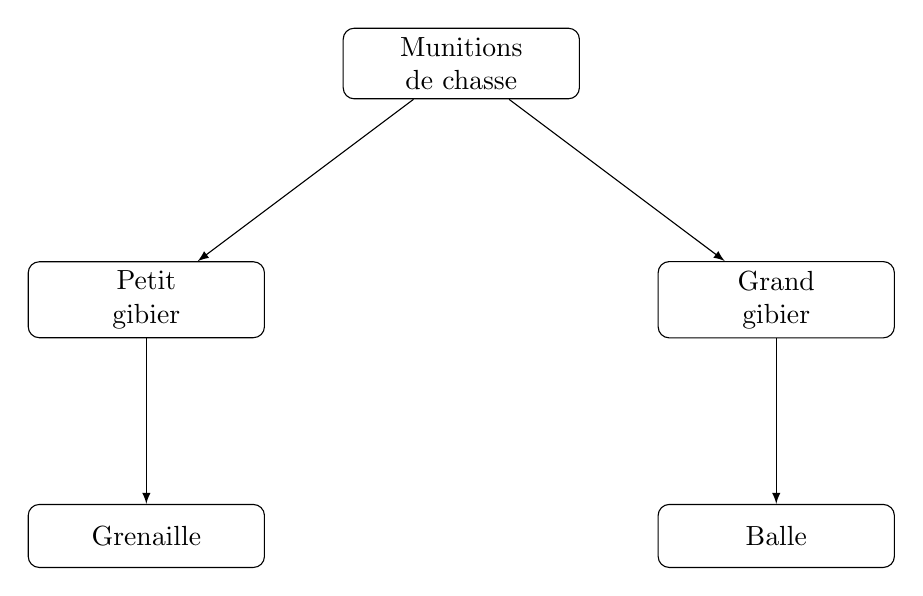
\begin{tikzpicture}[
every node/.style={
draw,
rounded corners,
align=center,
minimum width=3cm,
minimum height=8mm
}
]

\node (M) at (0,0) {Munitions\\de chasse};

\node (P) at (-4,-3) {Petit\\gibier};
\node (G) at (4,-3) {Grand\\gibier};

\node (Gr) at (-4,-6) {Grenaille};
\node (Ba) at (4,-6) {Balle};

\draw[-latex] (M) -- (P);
\draw[-latex] (M) -- (G);

\draw[-latex] (P) -- (Gr);
\draw[-latex] (G) -- (Ba);

\end{tikzpicture}

\caption{Exemples de munitions couramment utilisées selon le type de gibier.}
\label{fig:petit_grand_gibier}

\end{figure}

\section{Le petit gibier}

Le petit gibier comprend notamment :

\begin{itemize}
    \item certains oiseaux ;
    \item les lapins ;
    \item les lièvres ;
    \item divers petits mammifères.
\end{itemize}

Les cartouches à grenaille sont très largement utilisées dans ce domaine.

\section{Le grand gibier}

Le grand gibier regroupe notamment :

\begin{itemize}
    \item les sangliers ;
    \item les cervidés ;
    \item certains grands mammifères.
\end{itemize}

Les tirs sont généralement réalisés avec des projectiles uniques.

\section{Les cartouches à balle}

Les cartouches à balle utilisent un projectile unique.

Elles offrent généralement :

\begin{itemize}
    \item une meilleure portée ;
    \item une précision supérieure ;
    \item une énergie importante.
\end{itemize}

Elles sont principalement employées pour le grand gibier.

\section{Les cartouches à grenaille}

Les cartouches à grenaille contiennent un grand nombre de petits projectiles.

Après la sortie du canon, ceux-ci se dispersent progressivement.

Cette dispersion augmente les chances d'atteindre une cible de petite taille en
mouvement.

\begin{figure}[htbp]
\centering

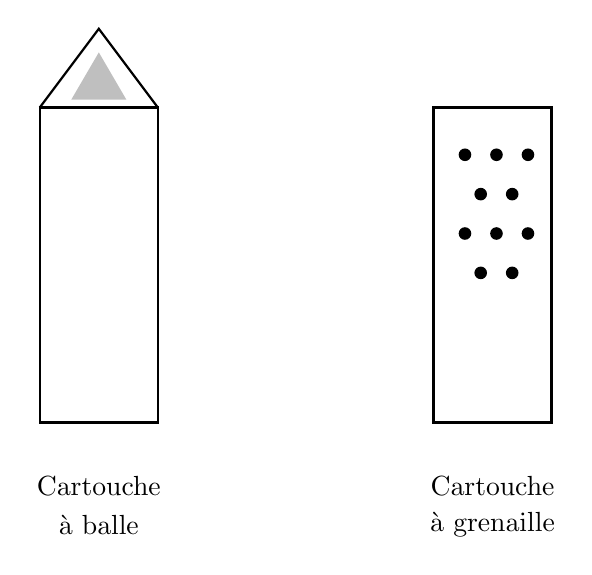
\begin{tikzpicture}[scale=1]

% Cartouche à balle
\draw[thick] (0,0) rectangle (1.5,4);
\draw[thick] (0,4) -- (0.75,5) -- (1.5,4);

\fill[gray!50] (0.4,4.1) -- (0.75,4.7) -- (1.1,4.1) -- cycle;

\node at (0.75,-0.8) {Cartouche};
\node at (0.75,-1.3) {à balle};

% Cartouche à grenaille
\begin{scope}[xshift=5cm]

\draw[thick] (0,0) rectangle (1.5,4);

\foreach \x/\y in {
0.4/3.4,0.8/3.4,1.2/3.4,
0.6/2.9,1.0/2.9,
0.4/2.4,0.8/2.4,1.2/2.4,
0.6/1.9,1.0/1.9
}
{
\fill (\x,\y) circle (0.08);
}

\node at (0.75,-0.8) {Cartouche};
\node at (0.75,-1.3) {à grenaille};

\end{scope}

\end{tikzpicture}

\caption{Comparaison simplifiée entre une cartouche à balle et une cartouche à grenaille.}
\label{fig:balle_grenaille}

\end{figure}

\section{La gerbe de plomb}

L'ensemble des projectiles dispersés est appelé :

\begin{quote}
gerbe
\end{quote}

La forme et la densité de cette gerbe influencent fortement l'efficacité du
tir.

\section{Influence de la distance}

Lorsque la distance augmente :

\begin{itemize}
    \item la gerbe s'élargit ;
    \item la densité d'impacts diminue ;
    \item l'énergie individuelle des projectiles diminue.
\end{itemize}

Le choix de la cartouche dépend donc fortement de la distance prévue.

\begin{figure}[htbp]
\centering

\begin{tikzpicture}[scale=1]

% Canon
\draw[thick] (0,0) -- (0,5);

\node[left] at (0,2.5) {Canon};

% Gerbes
\draw[dashed] (0,2.5) -- (3,3);
\draw[dashed] (0,2.5) -- (3,2);

\draw[dashed] (0,2.5) -- (6,4);
\draw[dashed] (0,2.5) -- (6,1);

\draw[dashed] (0,2.5) -- (9,5);
\draw[dashed] (0,2.5) -- (9,0);

% Distances
\draw (3,1.8) -- (3,3.2);
\node[below] at (3,1.8) {Courte};

\draw (6,0.8) -- (6,4.2);
\node[below] at (6,0.8) {Moyenne};

\draw (9,-0.2) -- (9,5.2);
\node[below] at (9,-0.2) {Longue};

\end{tikzpicture}

\caption{La gerbe s'élargit progressivement avec la distance.}
\label{fig:gerbe_distance}

\end{figure}

\section{Le calibre}

Dans le domaine du fusil de chasse, la notion de calibre diffère souvent de
celle rencontrée pour les armes rayées.

Les désignations les plus connues sont notamment :

\begin{itemize}
    \item calibre 12 ;
    \item calibre 16 ;
    \item calibre 20 ;
    \item calibre 28.
\end{itemize}

Leur signification sera étudiée plus loin dans l'ouvrage.

\section{La longueur de la chambre}

Les cartouches de chasse existent en plusieurs longueurs.

Le choix de la cartouche doit être compatible avec la chambre de l'arme.

\section{Les projectiles modernes}

Les projectiles de chasse modernes utilisent de nombreuses technologies :

\begin{itemize}
    \item noyaux plomb ;
    \item projectiles monolithiques ;
    \item conceptions expansives ;
    \item géométries optimisées.
\end{itemize}

\section{Expansion contrôlée}

De nombreuses balles de chasse sont conçues pour se déformer de manière
contrôlée après impact.

Cette déformation vise à améliorer le transfert d'énergie vers la cible.

\section{Préservation de la venaison}

Le chasseur cherche généralement à concilier :

\begin{itemize}
    \item efficacité ;
    \item sécurité ;
    \item préservation de la venaison.
\end{itemize}

Le choix du projectile influence directement ces critères.

\section{Sécurité}

La sécurité constitue un aspect fondamental de la chasse.

Le tireur doit tenir compte :

\begin{itemize}
    \item de son environnement ;
    \item de la portée potentielle du projectile ;
    \item des risques de ricochet ;
    \item de la présence éventuelle d'autres personnes.
\end{itemize}

\section{Évolution des réglementations}

Les réglementations relatives aux munitions de chasse évoluent régulièrement.

Certaines restrictions concernent notamment :

\begin{itemize}
    \item les matériaux utilisés ;
    \item les zones de chasse ;
    \item les espèces concernées.
\end{itemize}

\section{Vers les projectiles de chasse}

Les munitions de chasse utilisent une grande variété de projectiles adaptés à
des usages spécifiques.

Le chapitre suivant examinera plus en détail les principales familles de
projectiles utilisées dans ce domaine.

\begin{figure}[htbp]
\centering

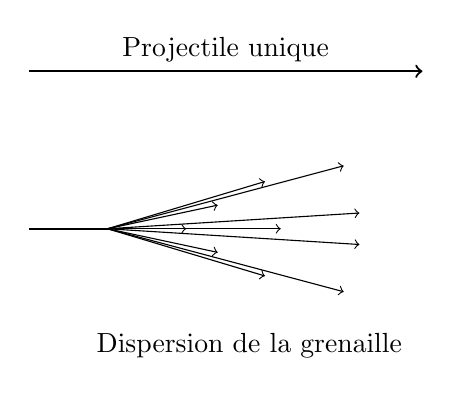
\begin{tikzpicture}[scale=1]

% Balle
\draw[thick,->] (0,0) -- (5,0);
\node[above] at (2.5,0) {Projectile unique};

% Grenaille
\begin{scope}[yshift=-2cm]

\draw[thick] (0,0) -- (1,0);

\foreach \x/\y in {
2/0,
2.4/0.3,
2.4/-0.3,
3/0.6,
3/-0.6,
3.2/0,
4/0.8,
4/-0.8,
4.2/0.2,
4.2/-0.2
}
{
\draw[->] (1,0) -- (\x,\y);
}

\node[below] at (2.8,-1.2) {Dispersion de la grenaille};

\end{scope}

\end{tikzpicture}

\caption{Différence de comportement entre un projectile unique et une charge de grenaille.}
\label{fig:balle_vs_grenaille}

\end{figure}

\section{À retenir}

\begin{aretenir}

\begin{itemize}
    \item Les munitions de chasse sont adaptées au type de gibier recherché.
    \item Les cartouches à balle et les cartouches à grenaille répondent à des
          besoins différents.
    \item La distance de tir influence fortement l'efficacité.
    \item Les projectiles modernes utilisent des conceptions variées.
    \item La sécurité reste une priorité absolue.
\end{itemize}

\end{aretenir}
